%%%%%%%%%%%%%%%%%%%%%%%%%%%%%%%%%%%%%%%%%%%%%%%%%%%%%%%%%%%%%%%%%%
%%%%%%%%%%%%%%%%%%%%%%%%%%%%%%%%%%%%%%%%%%%%%%%%%%%%%%%%%%%%%%%%%%

\subsection{Ports}
Un processeur \acrshort{IA-32} a la possibilité de transférer des données en utilisant
les ports d'entrée/sortie. Ces ports sont utilisés par le processeurs pour communiquer
avec des périphériques. Il peuvent être utilisés pour envoyer et recevoir des données
(par exemple un \textit{timer} va utiliser les ports d'entrée/sortie pour envoyer
son état). Les ports peuvent aussi être utilisés pour contrôler un péripéhrique
à partir de registres de contrôle (par exemple avec un controlleur de disque).\cite{ref64}
Etant donné que nous ne sommes pas sur du vrai \textit{hardware}, QEMU va se charger
d'émuler les différents périphériques utilisés par un processeur Intel 32-bits. \\

Les ports d'entrées/sorties sur architecture x86 se situent dans un espace d'adresses
séparé de la mémoire physique. Cet espace permet d'adresser 64000 (soit $2^{16}$)
ports de 8 bits. Les ports sont donc adressés sur 16 bits mais  il n'est pas possible
d'écrire dans un \acrshort{pio} de la même manière que l'on écrirait dans la mémoire
(avec une instruction  \mintinline{text}{MOV}) car nous sommes dans deux
espaces d'adresses différents. Ainsi, le \acrshort{cpu} utilise des instructions speciales
pour accéder aux \acrshort{pio}. Ces instructions sont les instructions
\mintinline{text}{IN} et \mintinline{text}{OUT}. \mintinline{text}{IN} permet de lire
tandis que \mintinline{text}{OUT} permet d'écrire. A noter que l'adresse du port
doit toujours être spécifiée dans le registre \mintinline{text}{dx} et la lecture
et l'écriture se font toujours avec les registres \mintinline{text}{ax/al}.\cite{ref42} \\

\begin{multicols}{2}
    [
    Exemple de lecture et d'écriture dans un port d'entrée/sortie :
    ]
    Ecrire 4 dans le port 0x2A :
    \begin{minted}[fontsize=\footnotesize,tabsize=4]{text}
        mov dx, 0x2A
        mov al, 4
        out dx, al
    \end{minted}
    \columnbreak
    Lire un octet depuis le port 0x2A :
    \begin{minted}[fontsize=\footnotesize,tabsize=4]{text}
        mov dx, 0x2A
        in  byte al, dx
    \end{minted}
\end{multicols}

Il existe une autre méthode pour écrire dans les ports utilisant le même bus d'adresse
pour la mémoire physique et pour les périphériques. Cette méthode consiste à
\textit{mapper} les ports d'entrées/sorties dans la mémoire physique (\acrshort{mmio}).
En écrivant dans la zone reservée aux ports, on écrirait alors directement dans
les ports et pas dans la mémoire physique. Le \textit{kernel} développé utilise
la première méthode (\acrshort{pio}).

%%%%%%%%%%%%%%%%%%%%%%%%%%%%%%%%%%%%%%%%%%%%%%%%%%%%%%%%%%%%%%%%%%
%%%%%%%%%%%%%%%%%%%%%%%%%%%%%%%%%%%%%%%%%%%%%%%%%%%%%%%%%%%%%%%%%%

\subsection{Interruptions et Exceptions}
\subsubsection{Principe général}
Les interruptions et les exceptions sont des évenements qui indiquent que l'attention
du processeur est demandée quelque part soit dans le code, soit par un périphérique.
Il existe deux types d'interruptions, les interruptions logicielles et les interruptions
matérielles. Les exceptions sont générées par le processeur mais diffèrent des
interruptions logicielles. Quand une interruption ou une exception a lieu, une
routine logicielle est appelée. Les processeurs Intel 32-bits supportent jusqu'à
256 interruptions seulement les 32 premiers numéros d'interruptions sont reservés
aux exceptions processeur.\cite{ref42} \\



\subsubsection{\acrshort{idt}}

%%%%%%%%%%%%%%%%%%%%%%%%%%%%%%%%%%%%%%%%%%%%%%%%%%%%%%%%%%%%%%%%%%
%%%%%%%%%%%%%%%%%%%%%%%%%%%%%%%%%%%%%%%%%%%%%%%%%%%%%%%%%%%%%%%%%%

\subsection{\acrshort{vga}}
Dans l'\acrshort{os} développé, le mode texte \acrshort{vga} a été utilisé pour
l'affichage. Toute carte graphique offre ce mode texte de 80 colonnes par 25 lignes.
Les 16 couleurs disponibles sont les suivantes :\cite{ref19}
\begin{figure}[!h]
  \centering
  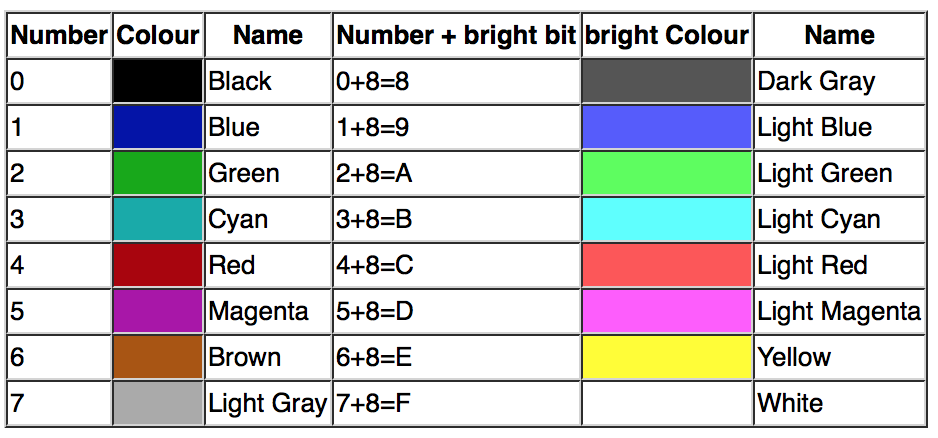
\includegraphics[scale=0.7]{images/colors.png}
  \caption{Couleurs du mode texte \acrshort{vga}}
\end{figure}

%%%%%%%%%%%%%%%%%%%%%%%%%%%%%%%%%%%%%%%%%%%%%%%%%%%%%%%%%%%%%%%%%%
%%%%%%%%%%%%%%%%%%%%%%%%%%%%%%%%%%%%%%%%%%%%%%%%%%%%%%%%%%%%%%%%%%

\subsection{\textit{Timer}}

%%%%%%%%%%%%%%%%%%%%%%%%%%%%%%%%%%%%%%%%%%%%%%%%%%%%%%%%%%%%%%%%%%
%%%%%%%%%%%%%%%%%%%%%%%%%%%%%%%%%%%%%%%%%%%%%%%%%%%%%%%%%%%%%%%%%%

\subsection{Clavier}